%%%%%%%%%%%%%%%%%%%%%%%%%%%%%%%%%%%%%%%%%%%%%%%%%%%%%%%%%%%%%%%%%%%%%%%%%%%%%%%%
\chapter{ПРОЕКТИРОВАНИЕ АРХИТЕКТУРЫ МОДУЛЯ}
%%%%%%%%%%%%%%%%%%%%%%%%%%%%%%%%%%%%%%%%%%%%%%%%%%%%%%%%%%%%%%%%%%%%%%%%%%%%%%%%

На рисунке \ref{image:architecture} изображена архитектура модуля. Опишем каждую часть модуля.

Первая часть, изображённая как getSipAccount, отвечает за получение данных о SIP-аккаунте пользователя. Вторая часть, изображённая как callEvents, передаёт серверу информацию о событиях звонка. Эта информация позволит web-приложению отображать текущие звонки и хранить историю о них. Данные этих двух частей отправляются AJAX-запросами на сервер. Третья часть отвечает за реализацию click-to-call.

\begin{figure}[h!]
\center{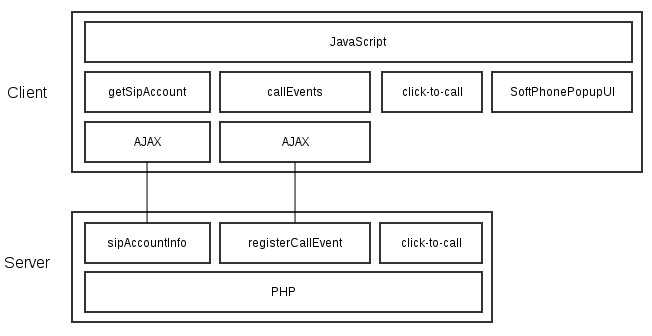
\includegraphics[width=0.8\linewidth]{architecture}}
\caption{Архитектура модуля}
\label{image:architecture}
\end{figure}



